% opis funkcjonalnosci aplikacji  

\section{Funkcjonalności aplikacji}
%TODO Opisać po skończeniu

Najistotniejsze funkcjonalności aplikacji to:
\begin{itemize}
    \item symulacja zachowania cieczy w zależności od zadanych warunków początkowych,
    \item możliwość przedefiniowania parametrów cieczy (gęstości, lepkości),
    \item możliwość obserwacji wyniku symulacji (położenia cząsteczek i~rozkładu ciśnień).
\end{itemize}

Do tej pory udało się nam już zasymulować zachowanie cieczy. Test poprawności napisanego algorytmu realizującego metodę \textit{SPH} przeprowadziliśmy w \textsf{Pythonie} (wizualizacja - rysunek \ref{fig:python}), a także w \textsf{C++} (dane liczbowe). Ponadto programowo dostępna jest zmiana wszystkich założonych parametrów cząsteczki cieczy. Podczas działania aplikacji w jej okienku obserwować można chaotycznie poruszające się cząsteczki cieczy. Rysunek \ref{fig:gui} przedstawia przykładowy zrzut ekranu działającej aplikacji.

\begin{figure}[H]
 \begin{center}
  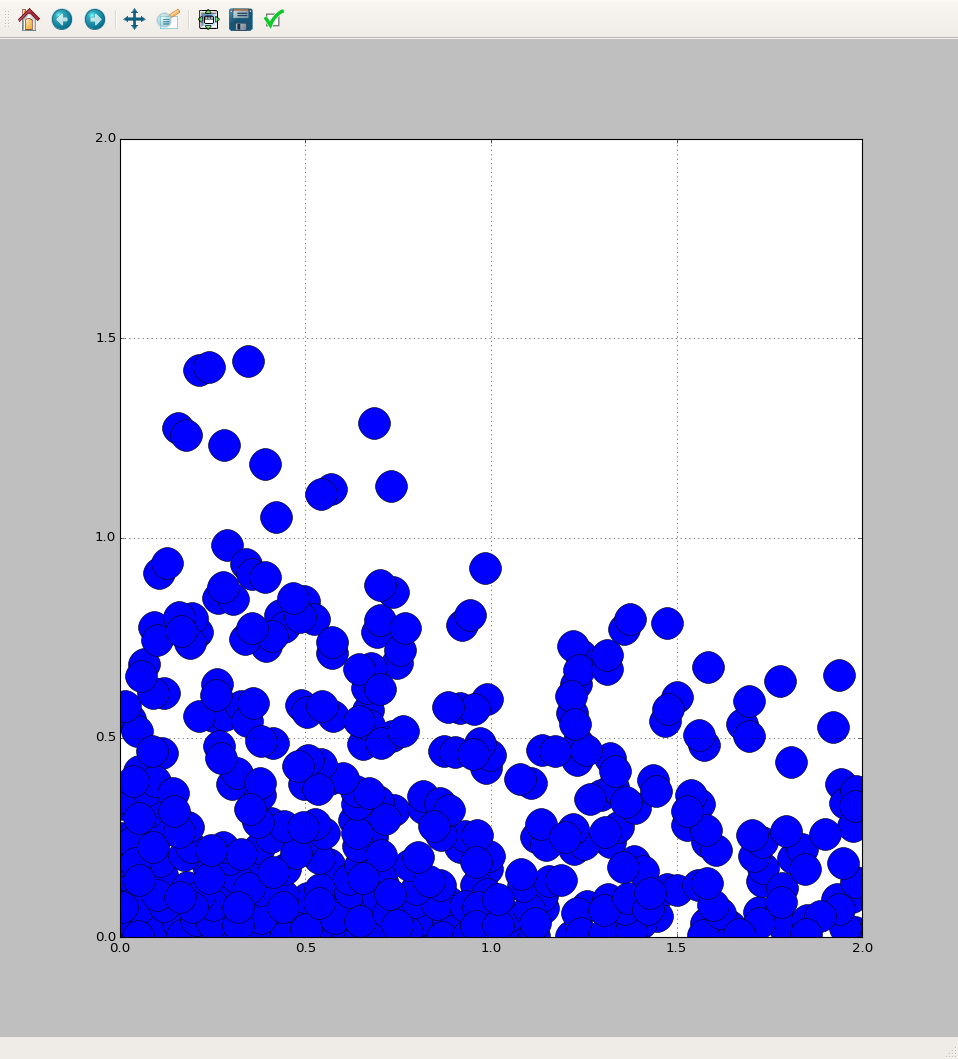
\includegraphics[width=0.7\textwidth]{rysunki/pythonViz.png}
 \end{center}
 \caption{Symulacja cieczy w Pythonie}
 \label{fig:python}
\end{figure}
